\documentclass[11pt]{article}
\usepackage[margin=1.5in]{geometry}
\usepackage{graphicx}
\usepackage{float}
\usepackage{parskip}
\usepackage{amsmath}
\usepackage{pgfplots}
\usepackage{subcaption}
\pgfplotsset{width=10cm, compat=1.9}

\begin{document}

\textbf{\Huge Applications of Integrals}

Athan Zhang \& Jeffrey Chen

\section{Basic Contextual Applications}
One of the most basic applications of integration lies in investigating the accumulation of change. In most cases, students will be given a function that models the rate of change of some quantity, and be asked to find the total change in the quantity. This can be done by finding the area under the function, or the integral of the function over some interval.


\section{Work}
Integration is extremely prevalent in physics. A good example of this is the concept of work. If a force $F$ is applied to an object in its direction of motion as it moves from point $x_0$ to $x_1$, then the \textbf{work} done on the object is defined as the following integral:

\[ W = \int_{x_0}^{x_1} F(x) dx \]

In some cases, the force applied may be constant, turning this integral into a simple multiplication. However, when the force varies as a function of the object's position, then the integral is necessary to account for the curve. There are many different formulas for force depending on the scenario, but the most commonly used and applicable one is Newton's second law of motion:

\[ F = ma \]

The mass of an object is usually constant (not always though), and when the force is varying, it is usually the acceleration that is causing the varying. For example, the acceleration could itself be a function of the object's position. In these cases, we must first derive a function for the force using Newton's second law of motion before being able to integrate the force to find work.

\section{Area Between Curves}
Students already know how to find the area under a single curve, but another application of integration lies in finding the area between two curves. For example, take the diagram below:

\begin{figure}[h]
    \centering
    \hspace*{0.7cm}   
    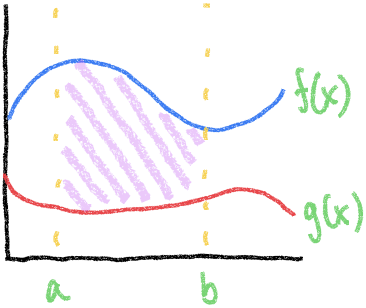
\includegraphics[width=0.3\textwidth]{Calculus/images/vertstack.png}
\end{figure}

In order to find the highlighted area between the two curves, we can utilize a technique similar to what we used for basic integration: splitting the area up into rectangles.

\begin{figure}[h]
    \centering
    \hspace*{2cm}    
    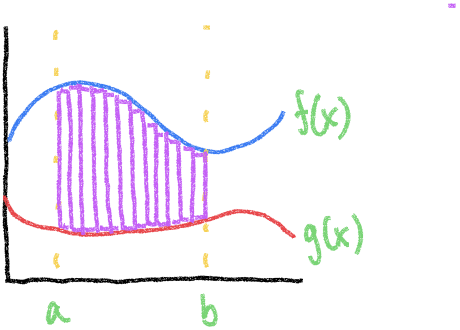
\includegraphics[width=0.4\textwidth]{Calculus/images/vertrect.png}
\end{figure}

From here on, this area problem is nearly identical to normal integration, except for one thing: the height of the rectangles. Here, instead of the height being the value of a single function at any given point, the height is the difference between the values of two functions. Therefore, we can write the area as the following integral:

\[ A = \int_{a}^{b}[f(x)-g(x)]dx \]

Now, what if the curves were set up in the reverse manner? More specifically, what if they were stacked horizontally instead of vertically, like in the diagram below?

\begin{figure}[h]
    \centering
    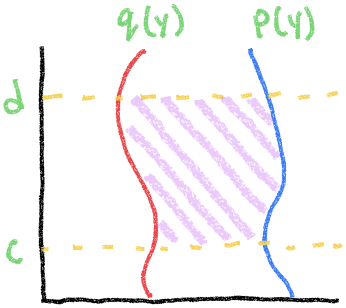
\includegraphics[width=0.3\textwidth]{Calculus/images/horstack.png}
\end{figure}

In this case, our previous method no longer works, as we cannot cleanly separate the area into vertical rectangles. However, if we simply rotate our rectangles to be horizontal, it fixes this issue:

\begin{figure}[h]
    \centering
    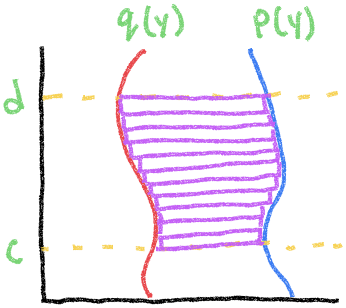
\includegraphics[width=0.3\textwidth]{Calculus/images/horrect.png}
\end{figure}

Note that the roles of the height and width have reversed now. In this case, the height of the rectangles is infinitesimally small, while the width of the rectangles depends on the horizontal difference between the functions. Finally, to sum the rectangles, we must integrate vertically instead of horizontally. This implies that the variable of integration must be $y$, not $x$. Thus, our integrand must also be in terms of $y$ and not $x$. To accomplish this, we must express the curves as functions of $y$ to produce the following formula:

\[ A = \int_{c}^{d}[p(y)-q(y)]dy \]

\section{Length of An Arc}
Integration can also be used to find the length of an arc or curve. The process for deriving this formula is a bit trickier than the previous ones, and it involves a theorem mentioned in an earlier unit.

First, we must recognize that the length of an arc can be approximated by splitting the arc into small sections and connecting the points with lines, as shown below:

\begin{figure}[h]
    \centering
    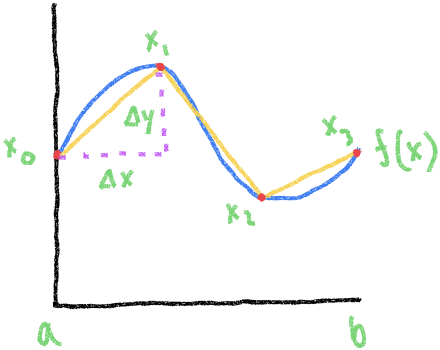
\includegraphics[width=0.4\textwidth]{Calculus/images/arc2.png}
\end{figure}

We can see that as the number of points and line segments increases, the total length of the line segments should approach the exact length of the arc. Let's investigate how to find that total length.

The length of the $k$th line segment should be equal to the following:
\[ L_k = \sqrt{(\Delta x_k)^2 + (\Delta y_k)^2}\]

The value of $\Delta x_k$ should be constant across all the line segments. The value of $\Delta y_k$ can be written as $f(x_k)-f(x_{k-1})$. Finally, we can write the total length of the line segments as a limit of a summation:

\[ L = \lim_{n \to \infty} \sum_{k=1}^n \sqrt{(\Delta x_k)^2 + (f(x_k)-f(x_{k-1}))^2}\]

Now, the Mean Value Theorem states that between every two adjacent points $x_k$ and $x_{k-1}$, there is a point $x_m$ where the following is true:

\[ f'(x_m) = \frac{f(x_k)-f(x_{k-1})}{x_k-x_{k-1}} = \frac{f(x_k)-f(x_{k-1})}{\Delta x_k}\]

We can rearrange into the following:

\[ f(x_k)-f(x_{k-1}) = \Delta x_k f'(x_m) \]

Next, we can substitute this expression into our earlier formula for $L$ and simplify:

\[ L = \lim_{n \to \infty} \sum_{k=1}^n \sqrt{(\Delta x_k)^2 + (\Delta x_k f'(x_m))^2} = \lim_{n \to \infty} \sum_{k=1}^n \sqrt{1 + ( f'(x_m))^2} \Delta x_k\]

Finally, as $\Delta x_K$ becomes infinitesimally small, we can convert this limit of a sum into an integral:

\[ L = \int_{a}^{b} \sqrt{1+ (f'(x))^2} dx\]

Thus, we have derived a formula for the length of any smooth curve on the interval $[a, b]$.

\section{Surface Area}
The ability to find the lateral surface area of any solid created by \textbf{revolution} stems directly from the formula for the length of an arc. A solid formed by \textbf{revolution} can be sliced into to find a cross section, and can then be represented by the revolution of that cross section around an axis, as shown in the example below.

\begin{figure}[h]
    \hspace*{2cm}
    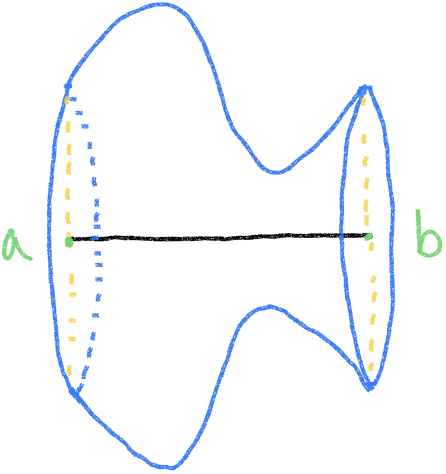
\includegraphics[width=0.3\textwidth]{Calculus/images/revolution.png}
    \hspace*{2cm}
    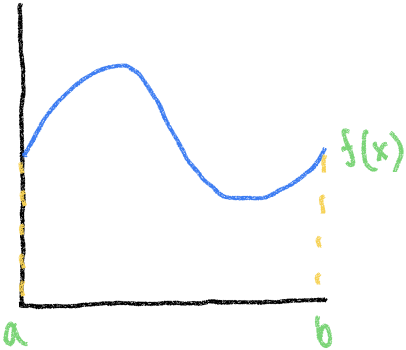
\includegraphics[width=0.3\textwidth]{Calculus/images/section.png}
\end{figure}

To find the surface area of the resulting solid, we can integrate the length of the outer surface of the cross section over the revolution of the axis. The length of interest can be simply found using the arc length formula from the previous section. In order to adjust for the revolution of the length, we can simply multiply the integrand by the circumference of the revolution at each point, to obtain the following formula:

\[ A_{\textit{lateral}} = \int_{a}^{b} 2\pi f(x) \sqrt{1+(f'(x))^2} dx\]


\section{Volume}
Similar to how integrals can be applied to find the surface area of solids, we can also use them to determine volumes. There are two primary methods of doing this, both of which will be covered below. In some scenarios, these two methods both work, but in most cases it will require some intuition to pick the correct method to use.

\subsection{Basic Method}
First, we must come up with a conceptual plan as to how we will integrate the volume of a solid. Remember that integration can be thought of as the sum of many small parts. Recall that we broke areas down into infinitely many thin rectangles to integrate them. For volume, we can think of a similar method. 

Instead of thin rectangles, we can split a solid into infinitely many thin cross sections and sum them up to produce the volume of the solid, as shown below: 

\begin{figure}[H]
    \centering
    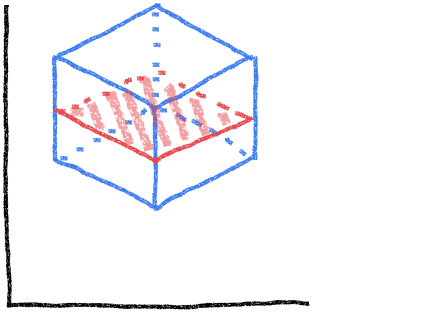
\includegraphics[width=0.4\textwidth]{Calculus/images/crosssection.png}
\end{figure}

Recall that the integral for the area under a curve was the following:

\[ \int_{a}^{b} f(x) dx \]

In this integral, $f(x)$ represented the height of each rectangle, while $dx$ represented the infinitesimally small width of each rectangle. The integral sign simply represented the infinite sum of the product of these two quantities, otherwise known as the area of each rectangle. 

Using similar lagic, if we integrate the volume of every thin cross section, we should obtain the volume. If a cross section is thin enough, the dimensions of the top and bottom faces should be essentially identical. Therefore, we can represent the volume as that of a simple solid:

\[ V_{\textit{slice}} = A(x) dx \]

In this formula, $A(x)$ represents a general formula for the area of the face of the cross section, while $dx$ represents the infinitesimally small height. Now, we can integrate this expression to obtain a general formula for the volume of a solid:

\[ V = \int_{a}^{b} A(x) dx \]

\subsection{Disks and Washers}
In the case of solids of revolution, we can express $A(x)$ rather easily. Take the following solid and its function of revolution:

\begin{figure}[H]
    \hspace*{2cm}
    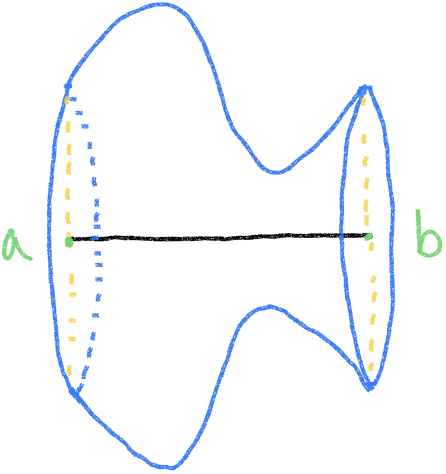
\includegraphics[width=0.3\textwidth]{Calculus/images/revolution.png}
    \hspace*{2cm}
    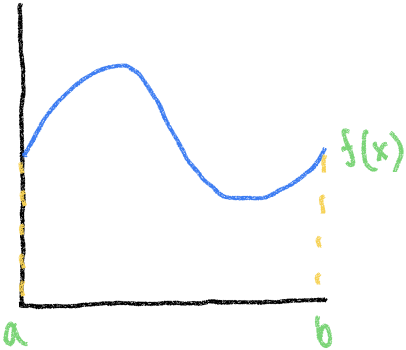
\includegraphics[width=0.3\textwidth]{Calculus/images/section.png}
\end{figure}

Here, we can observe that each cross section is a simple \textbf{disk} (hence \textbf{disk method}) of radius $f(x)$, as shown below:

\begin{figure}[H]
    \hspace*{2cm}
    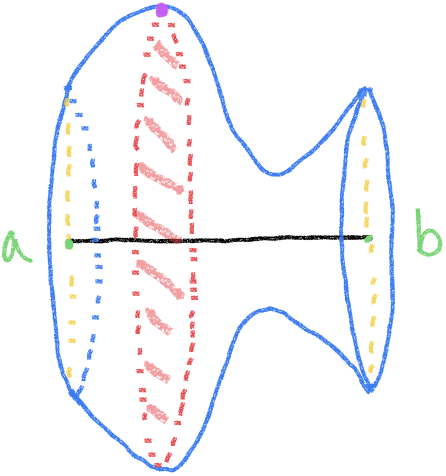
\includegraphics[width=0.3\textwidth]{Calculus/images/solidsectiondisk.png}
    \hspace*{2cm}
    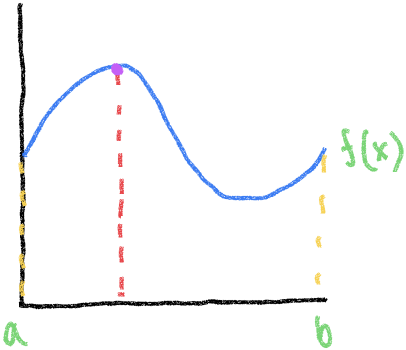
\includegraphics[width=0.3\textwidth]{Calculus/images/functionsectiondisk.png}
\end{figure}

Therefore, our previous vague formula $A(x)$ can be specifically defined as:

\[ A(x) = \pi [f(x)]^2 \]

Thus, the volume of a solid of revolution (with no holes in it) is given by:

\[ V = \int_{a}^{b} \pi [f(x)]^2 dx \]

Notice the specification of no holes in the solid. This is due to the fact that if there are holes, then the cross section is no longer a disk. Let us investigate this a bit further. Take the following solid and its functions of revolution:

\begin{figure}[H]
    \hspace*{2cm}
    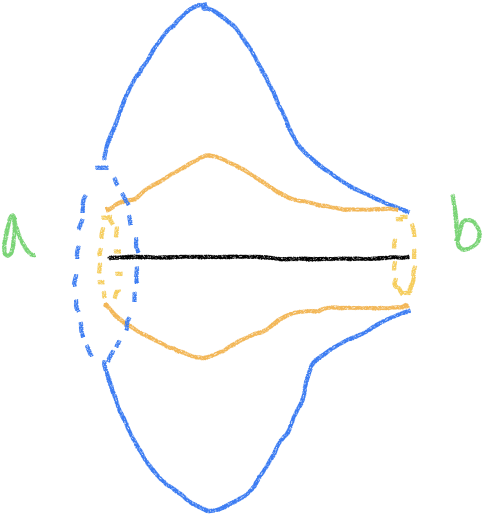
\includegraphics[width=0.3\textwidth]{Calculus/images/washersolid.png}
    \hspace*{2cm}
    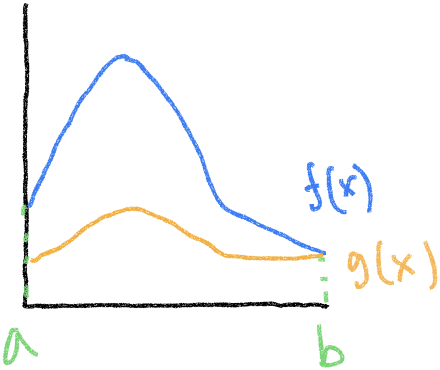
\includegraphics[width=0.3\textwidth]{Calculus/images/washerfunction.png}
\end{figure}

Notice the cross section of this solid looks more like a donut, or \textbf{washer} (hence \textbf{washer method}):

\begin{figure}[H]
    \hspace*{2cm}
    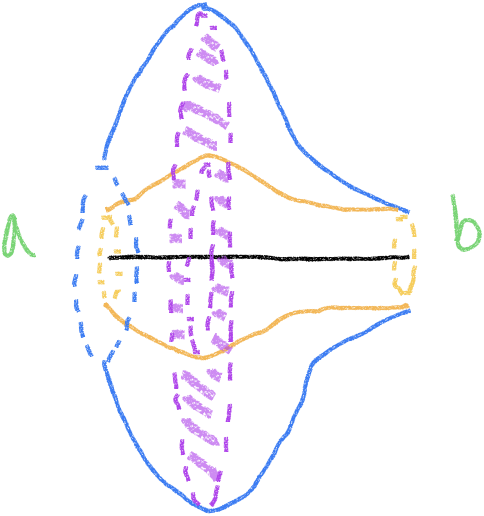
\includegraphics[width=0.3\textwidth]{Calculus/images/solidsectionwasher.png}
    \hspace*{2cm}
    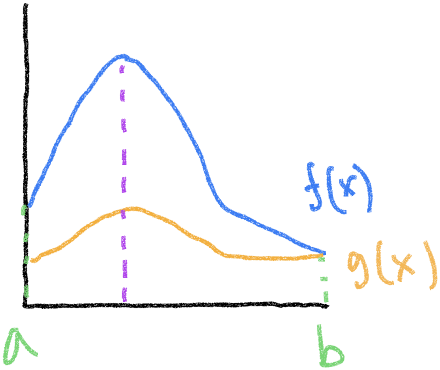
\includegraphics[width=0.3\textwidth]{Calculus/images/functionsectionwasher.png}
\end{figure}

The surface of the cross section is now an annulus of radii $f(x)$ and $g(x)$. Therefore, we can define the area $A(x)$ as:

\[ A(x) = \pi ([f(x)]^2 - [g(x)]^2) \]

Thus, the volume of a solid of revolution with a hole in it is given by:

\[ V = \int_{a}^{b} \pi ([f(x)]^2 - [g(x)]^2) dx \]
 
\subsection{Shells}

The second method of finding volume differs from the disk and washer method in the orientation of the thin slices we make. Given a solid of revolution, we can determine a function of revolution and an axis of rotation. 

In the disk and washer method, we take thin slices of the function \textbf{perpendicular} to the axis of rotation, thus creating the thin disk and washer shapes we are familiar with.

However, if we instead take thin slices of the function \textbf{parallel} to the axis of rotation, we then integrate a different portion of the solid:

\begin{figure}[h]
    \hspace*{2cm}
    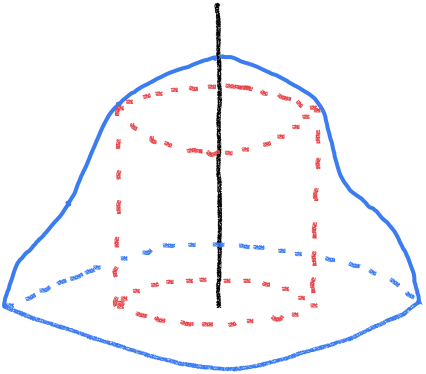
\includegraphics[width=0.3\textwidth]{Calculus/images/solidshell.png}
    \hspace*{2cm}
    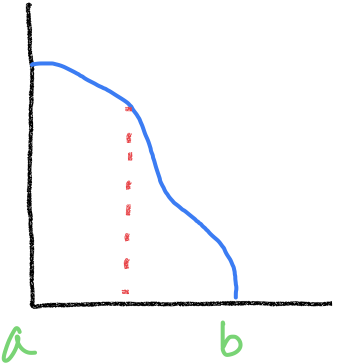
\includegraphics[width=0.3\textwidth]{Calculus/images/functionshell.png}
\end{figure}

The resulting portions of the solid are thin layers or \textbf{shells} of the solid (hence \textbf{shell method}). Thus, instead of integrating thin slices from end to end, we integrate thin shells from inside out. The volume of a thin shell can be expressed as: 

\[ V &= \text{[area of cross section]} \cdot \text{[height]} \]
\[ &= (\pi r_1^2 - \pi r_2^2)h \]
\[ &= \pi (r_1+r_2)(r_1-r_2)h \]
\[ &= 2\pi \frac{1}{2}(r_1+r_2)(r_1-r_2)h\]

We can observe that $\frac{1}{2}(r_1+r_2)$ is the average of the two radii, and $(r_1-r_2)$ is the difference between the two. As the shell becomes more and more thin and value of the radii become closer and closer, the average of the radii approaches $x$, while the difference becomes infinitesimally small, or $dx$. Finally, $h$ is simply $f(x)$. Therefore, we can replace those variables and transform this into an integral:

\[ V = \int_a^b 2\pi x f(x) dx \]

Thus, we have a formula for the volume of a solid using cylindrical shells.

\end{document}